\documentclass[12pt,pdftex,a4paper]{article}
\usepackage[english]{babel}
\usepackage{amsmath}
\usepackage{amssymb}
\usepackage{bbm}
\newcommand{\bbN}{\mathbbm{N}}
\newcommand{\bbR}{\mathbbm{R}}
\newcommand{\bbZ}{\mathbbm{Z}}
\newcommand{\bbI}{\mathbbm{I}}
\usepackage[pdftex]{graphicx}
\usepackage{listings}
\lstset{language=Python,basicstyle=\footnotesize}
\begin{document}
\title{Practical Course Robotics\\Weekly Summary}
\author{Mohammed Muddasser, Raphael Broesamle}
\date{Calendar week 27}
\maketitle
%%%%%%%%%%%%%%%%%%%%%%%%%%%%%%%%%%%%%%%%%%%%%%%%

\section*{Achievements this week}
\begin{itemize}
\item
Work Package 1 - Scene Creation:
Improvements to the scene so as to improve the visual appeal. New meshes added for the goal and fences. Work Package 1 is now complete.
\\
\begin{enumerate}
    \begin{minipage}{\linewidth}
        \centering
        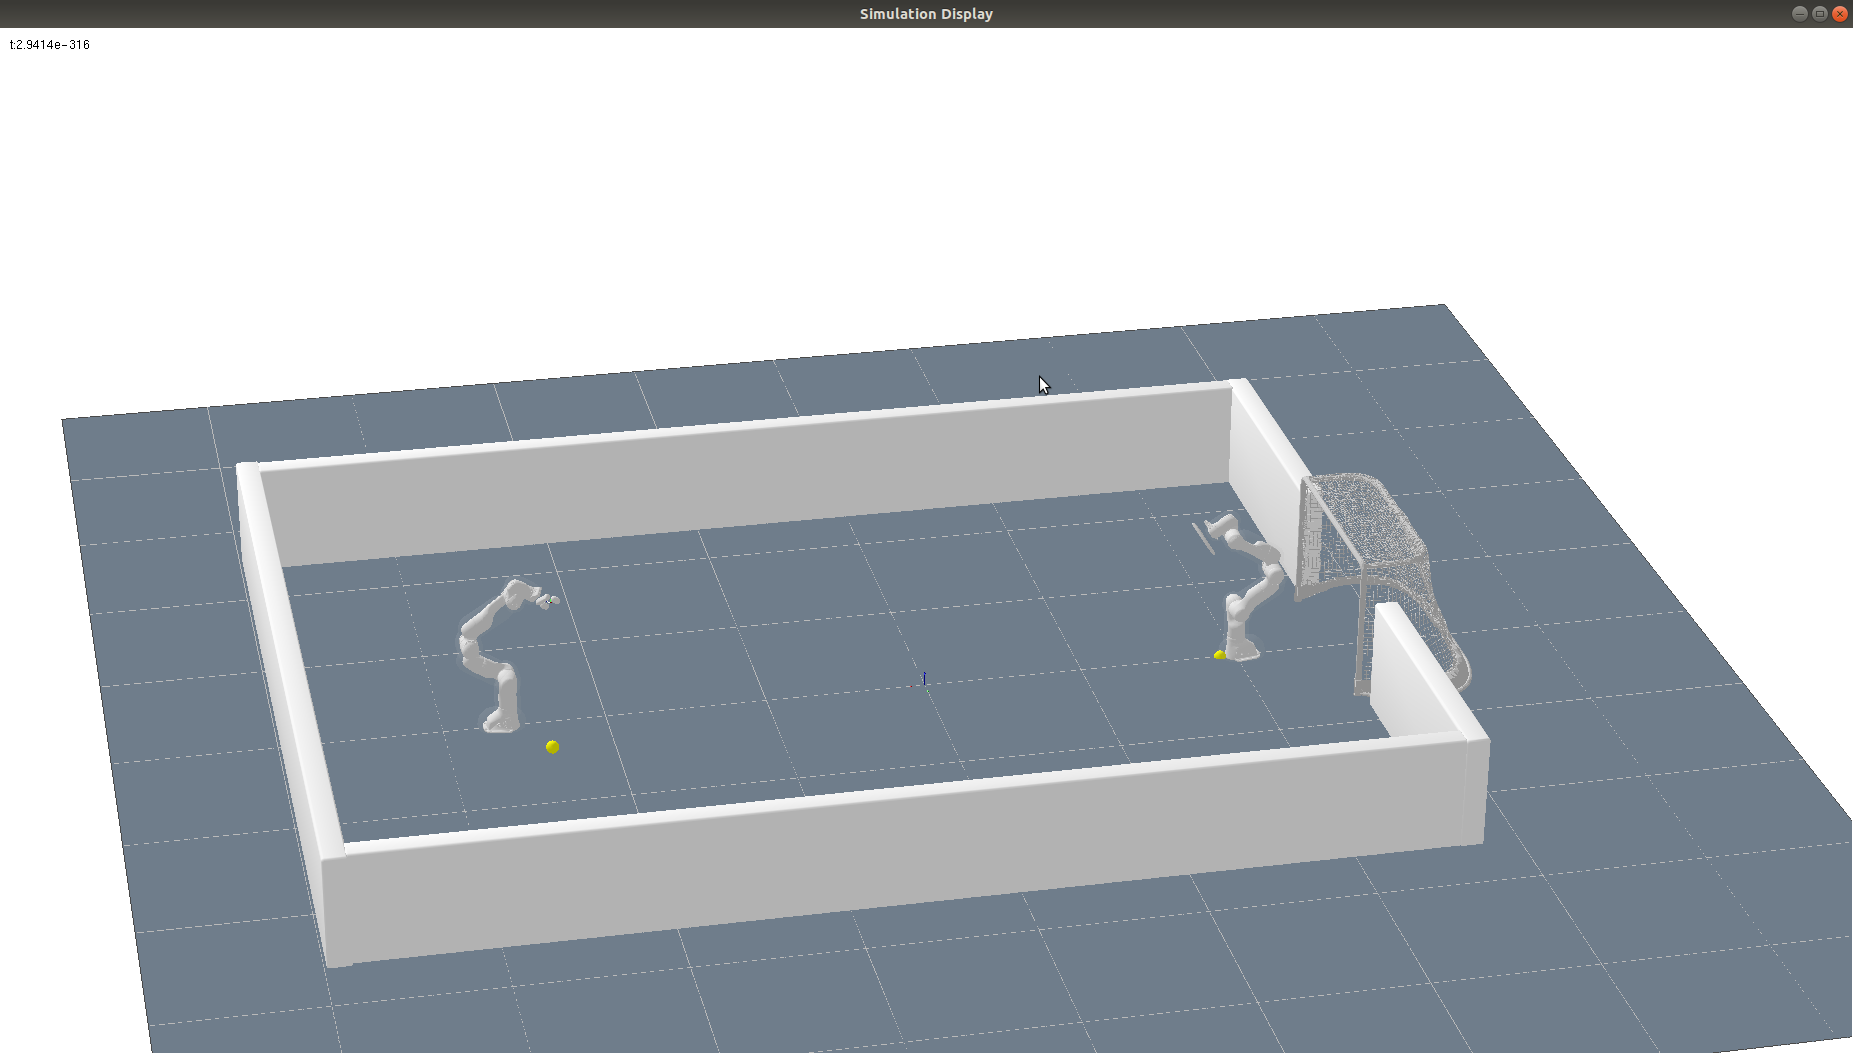
\includegraphics[width=0.75\textwidth]{environment.png}
        \captionof{\\Scene}
    \end{minipage}
\end{enumerate}

\item
Work Package 3 - Trajectory planning:
The Ball Management is now complete with trajectory estimation for the projectile which includes the estimation of the point of intersection between the ball and the goalie.
\\
\begin{enumerate}
    \begin{minipage}{\linewidth}
        \centering
        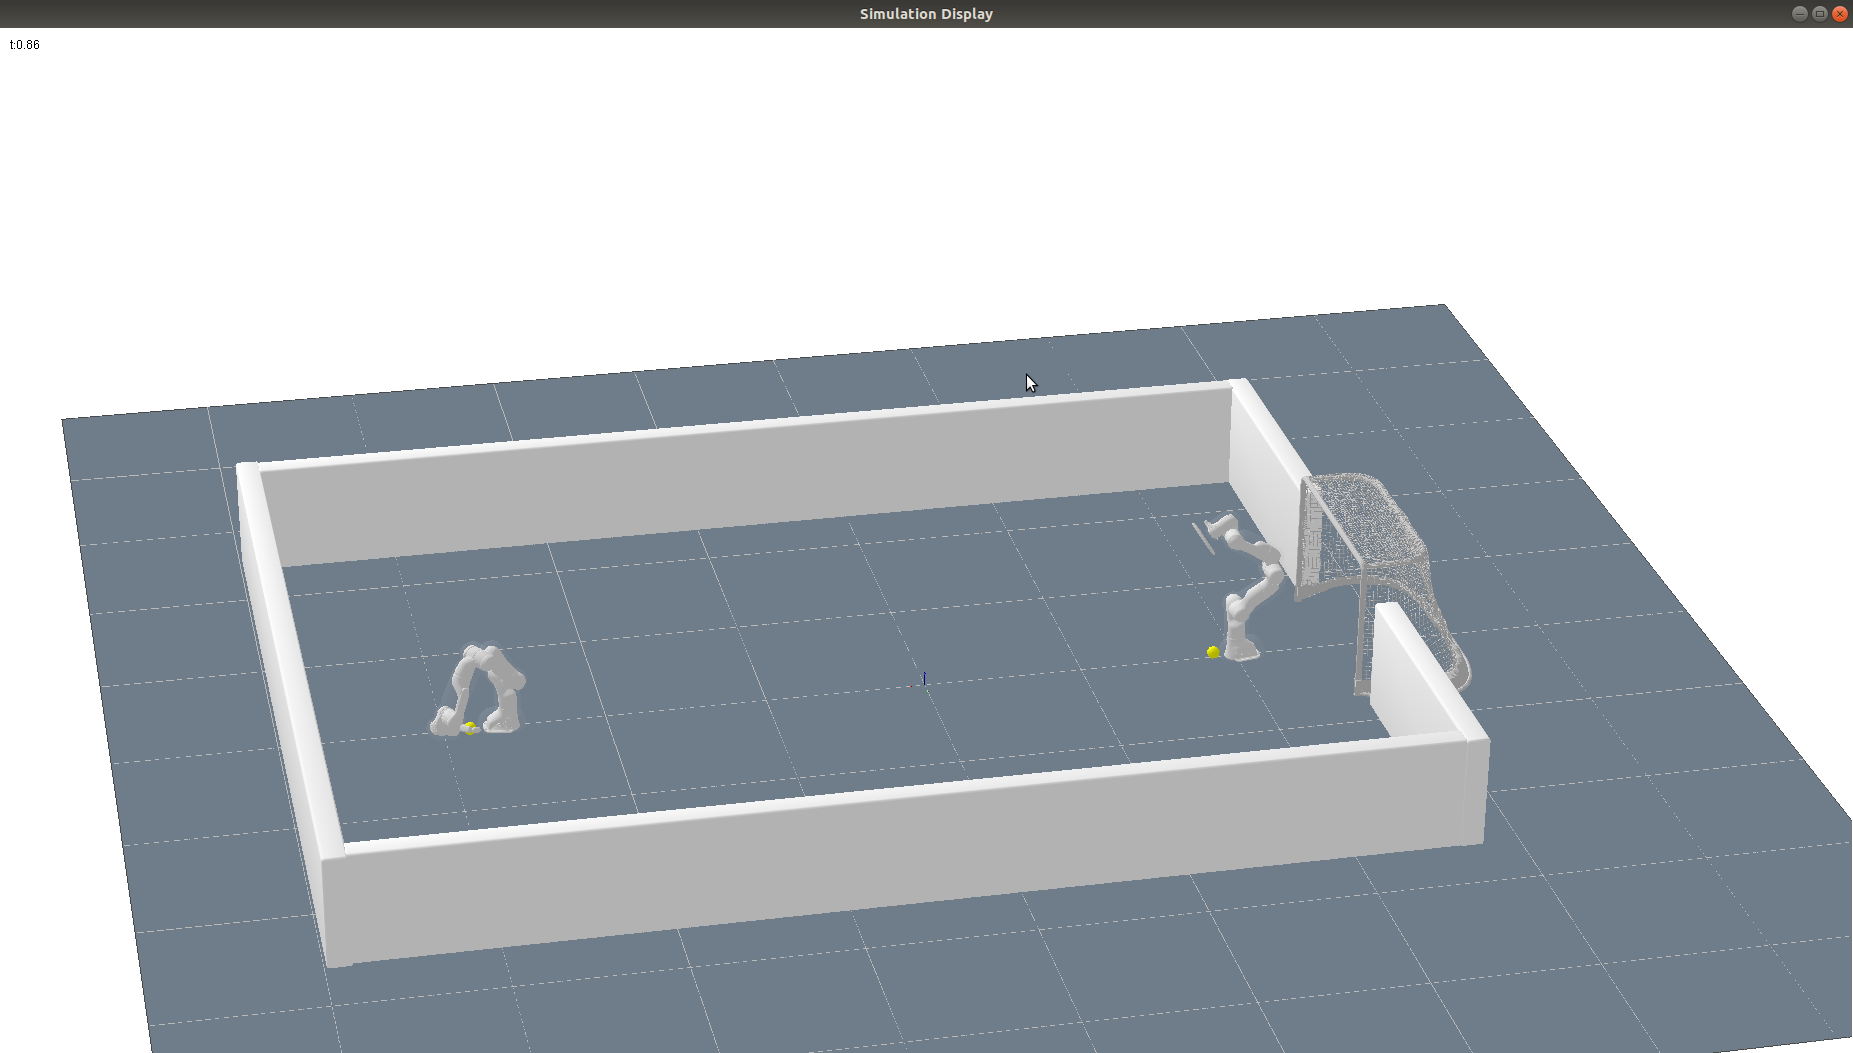
\includegraphics[width=.6\textwidth]{throw1.png}
        \captionof{\\}
        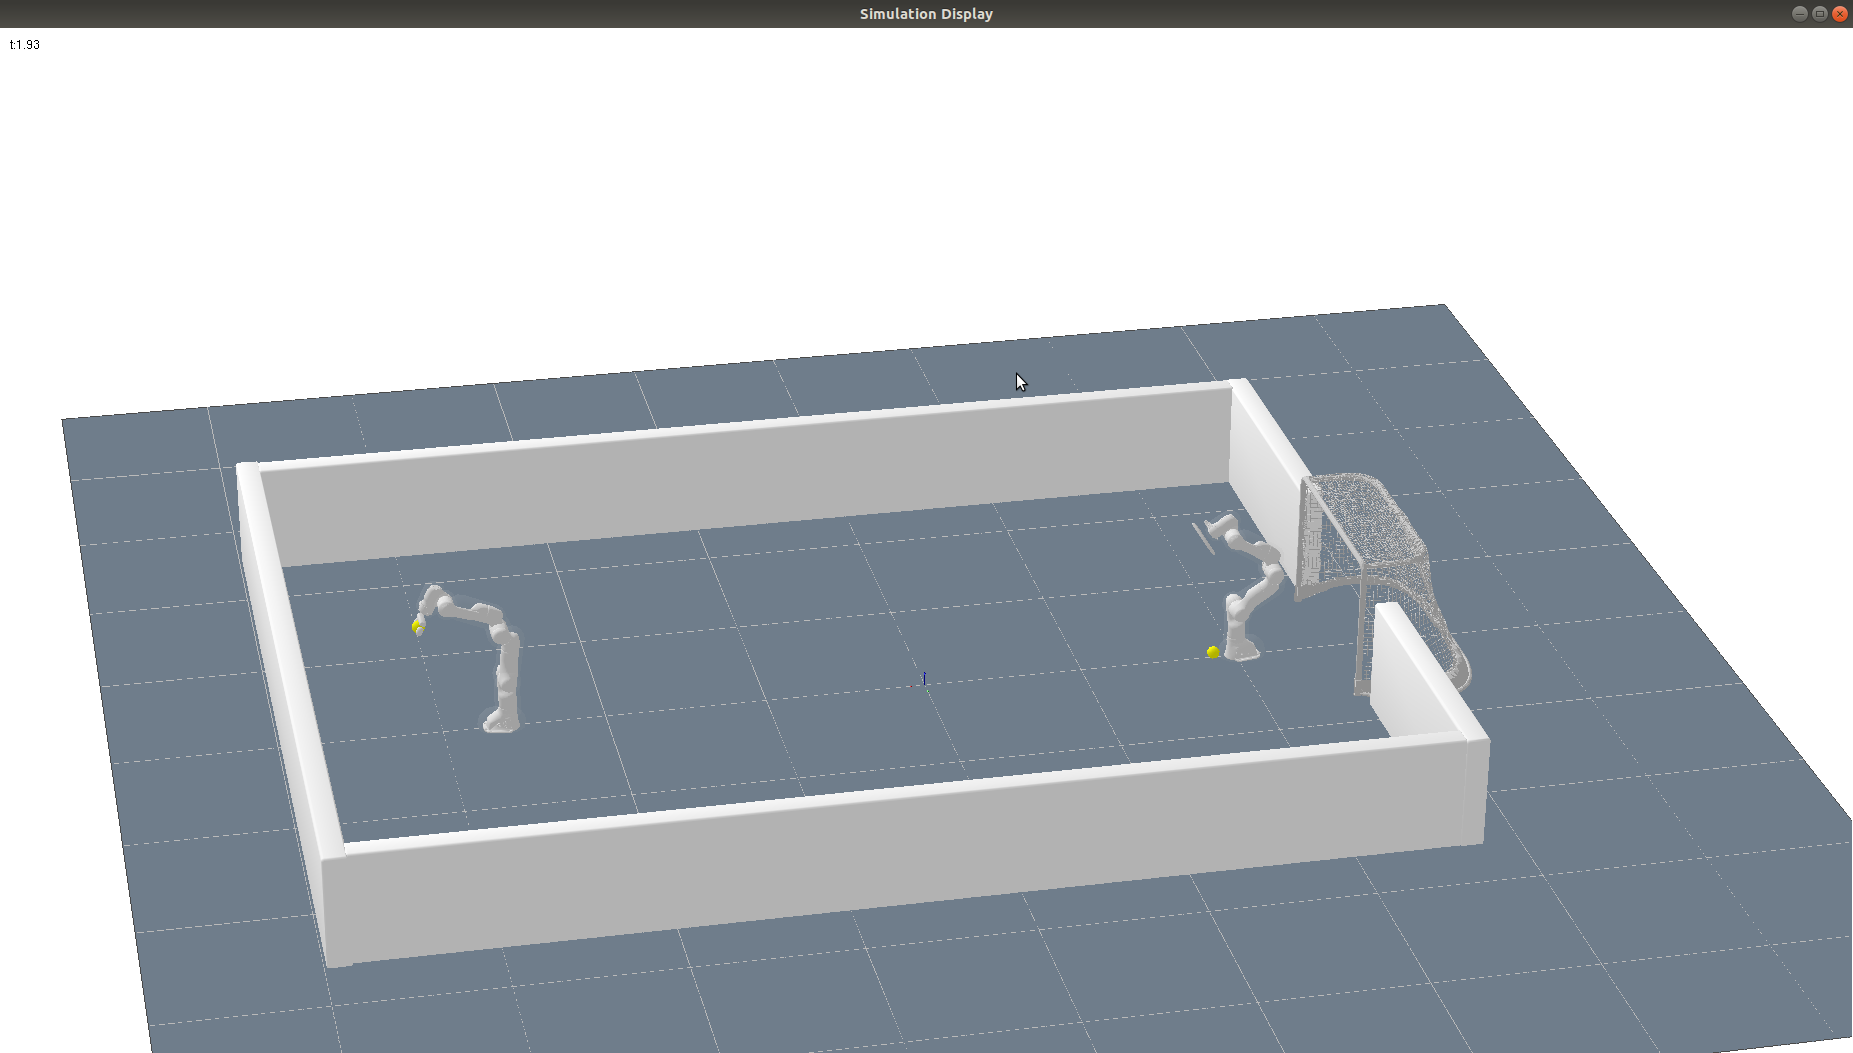
\includegraphics[width=.6\textwidth]{throw2.png}
        \captionof{\\}
        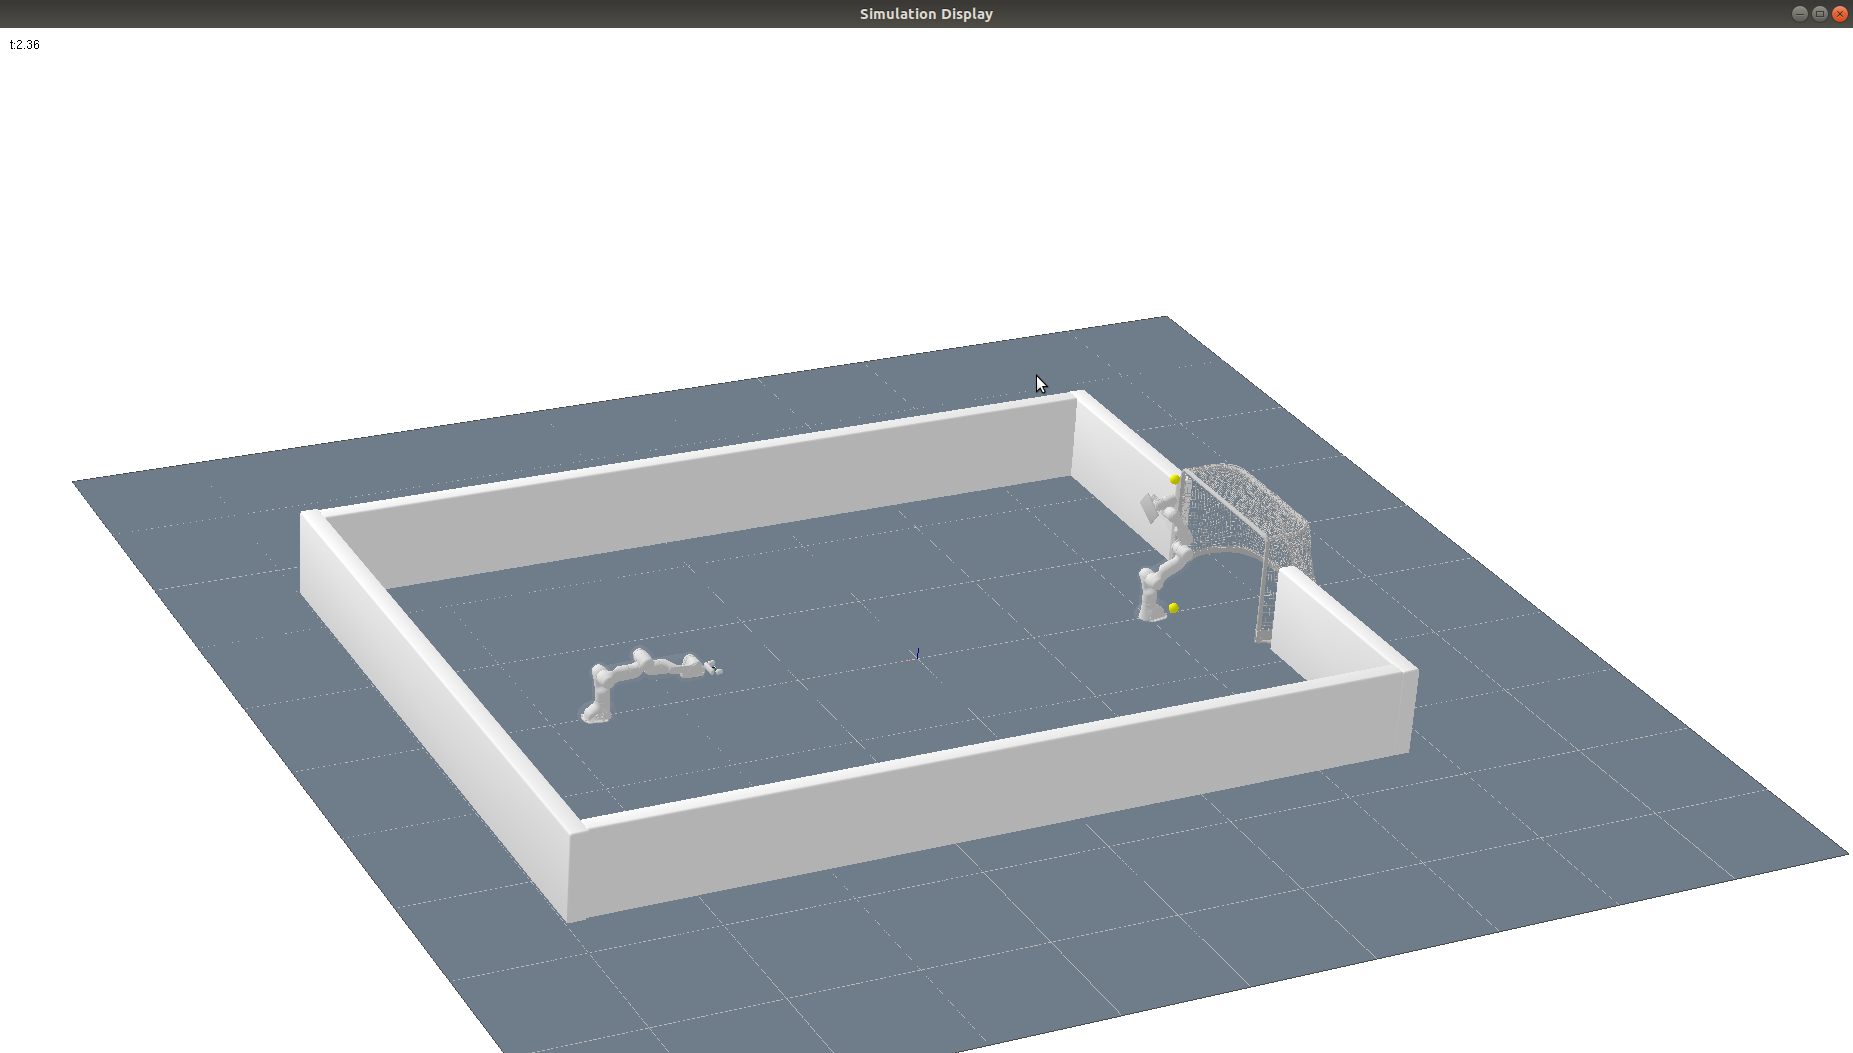
\includegraphics[width=.6\textwidth]{trajectory.png}
        \captionof{\\Trajectory planning}
    \end{minipage}
\end{enumerate}

\item
Work Package 4 - Goalie:
The objectives to move the goalie to the desired position have been implemented separately. But not yet integrated with the whole environment.
\end{itemize}

\section*{Goals for next week}
\begin{itemize}
\item
Work Package 5 - Integration and Extensive Testing:
Integration of the work packages and testing the various scenarios. Defining and calibrating the objective functions and various parameters to get the best results. Structuring the code and documentation. 
\item
Work Package 6 - Video and Presentation preparation\end{itemize}

%%%%%%%%%%%%%%%%%%%%%%%%%%%%%%%%%%%%%%%%%%%%%%%%
\end{document}

